\documentclass[10pt]{article}


\usepackage[lmargin=2cm, rmargin=2cm, top=1.5cm, bottom=1.5cm]{geometry}
\usepackage{longtable,multirow,booktabs}
\usepackage{mathrsfs} % para formato de letra
\usepackage[spanish]{babel}
\usepackage[utf8]{inputenc}
\usepackage{amsmath}
\usepackage{amsfonts}
\usepackage{amssymb}
\usepackage{graphicx}
\usepackage{tikz}
\usepackage{float}
\usepackage{dsfont}%Sirve para poner el simbolo de los reales
\graphicspath{imagenes}
\usepackage{hyperref}


\title{\bfseries \huge {Apuntes de Django} }
\author{Ezequiel Remus: $<ezequielremus@gmail.com>$}
\date{}

%%%%%%%%%%%%%%%%%%%%%%%%%%%%%%%%%%%%%%%%%%%%%%%%%%%%%%%%%%%%%%%%
%						Ayudas                                 %
%%%%%%%%%%%%%%%%%%%%%%%%%%%%%%%%%%%%%%%%%%%%%%%%%%%%%%%%%%%%%%%%

%\textcolor{LimeGreen}{Hola}
%\colorbox{LimeGreen}{Hola}
%\fcolorbox{LimeGreen}{White}{Hola}
%\fcolorbox{Black}{LimeGreen}{Hola}

%\definecolor{Micolor1}{RGB}{193,124,250}
%\textcolor{Micolor1}{Hola}

%%%%%%%%%%%%%%%%%%%%%%%%%%%%%%%%%%%%%%%%%%%%%%%%%%%%%%%%%%%%%%%%

%%%%%%%%%%%%%%%%%%%%%%%%%%%%%%%%%%%%%%%%%%%%%%%%%%%%%%%%%%%%%%%%
%			 	  Definciciones de Variables                   %
%%%%%%%%%%%%%%%%%%%%%%%%%%%%%%%%%%%%%%%%%%%%%%%%%%%%%%%%%%%%%%%%
%%%%%%%%%%%
% COLORES %
%%%%%%%%%%%
\definecolor{R}{RGB}{176, 11, 11}
\definecolor{B}{RGB}{52, 75, 201}
\definecolor{G}{RGB}{20, 176, 18}
\definecolor{M}{RGB}{133, 71, 33}

%%%%%%%%%%%
%  TEXTO  %
%%%%%%%%%%%
\newcommand{\py}[1]{{\textcolor{B}{Python} #1}}
\newcommand{\django}[1]{{\textcolor{G}{Django} #1}}
\newcommand{\titulo}[1]{\textcolor{R} #1}

%%%%%%%%%%%%%%%%%%%%%%%%%%%%%%%%%%%%%%%%%%%%%%%%%%%%%%%%%%%%%%%%
%						Inicio del documento                   %
%%%%%%%%%%%%%%%%%%%%%%%%%%%%%%%%%%%%%%%%%%%%%%%%%%%%%%%%%%%%%%%%

\begin{document}
\renewcommand{\tablename}{Tabla}
%\pagestyle{myheadings}
%TITULO
%modificar el formato del titulo
\maketitle
\newpage
\section*{Resumen}

Este documento esta basado en la documentación de \django{}.
En particular corresponde a la version Django 3.0, que admite Python 3.6 y versiones posteriores.  
\tableofcontents
\newpage
\section{Introducción}
\subsection{¿Que es Django?}

\django{} es un framework web diseñado para realizar aplicaciones de cualquier complejidad en unos tiempos muy razonables.

Está escrito en \py{} y tiene una comunidad muy amplia, que está en continuo crecimiento

\subsection{¿Porqué usarlo?}

Los motivos principales para usar \django{} son:
 
\begin{itemize}

\item Es muy rápido : Si tenés una startup, estas apurado por terminar un proyecto proyecto o, simplemente, querés reducir costes, con \textit{\django{} podéis construir una aplicación muy buena en poco tiempo.}
 
 \item Viene bien cargado : Cualquier cosa que necesitéis realizar, ya estará implementada, sólo hay que adaptarla a vuestras necesidades. Ya sea porque hay módulos de la comunidad, por cualquier paquete \py{} que encontréis o las propias aplicaciones que \django{} trae, que son muy útiles.
 
 \item Es bastante seguro : Podemos estar tranquilos con \django{}, ya que implementa por defecto algunas medidas de seguridad, las más clásicas, para que no haya \textbf{SQL Injection}, no haya \textit{Cross site request forgery} \textbf{(CSRF)} o no haya \textbf{Clickjacking} por \textit{JavaScript}. \django{} se encarga de manejar todo esto de una manera realmente sencilla.
 
 \item Es muy escalable : Podemos pasar desde muy poco a una aplicación enorme perfectamente, una aplicación que sea modular, que funcione rápido y sea estable.
 
 \item Es increíblemente versátil : Es cierto que en un principio \django{} comienza siendo un Framework para almacenar noticias por sitios de prensa, blogs y este estilo de webs, pero con el tiempo ha ganado tanta popularidad que se puede usar para el propósito que queráis.
\end{itemize}

\textit{Otras bondades de \django{} que no se destacan en la web son:}

Su \textbf{ORM}, su interfaz para acceso a la base de datos , ya que hacer consultas con ella es una maravilla, es una herramienta muy buena.

Trae de serie un panel de administración, con el cual podemos dejar a personas sin ningún tipo de conocimiento técnico manejando datos importantes de una forma muy cómoda


\section{Iniciando un proyecto}
\subsection{Entornos Virtuales}
Lo primero y más importante es asegurarnos de crear un entorno para trabajar en nuestro proyecto.

Un entorno virtual es básicamente una abstracción la cual crea un conjunto vacío en \py{}, donde solo esta instalada la versión de \py{} que se utiliza junto con \textbf{pip} y las librerías básicas. En este conjunto podremos instalar todas las librerías que utilizaremos en el proyecto. Esto nos permitirá crear luego un archivo de referencia para conocer las librerias y versiones de estas utilizadas por el proyecto. 

Existen varias formas de crear entornos virtuales: 
%%%%%%%%%%%%%%%%%%%%%%%%%%%%%%%%%%%%%%%%%%%%%%%%%%%%%%%%%%%%%%%%
%						ITEMIZE                                %
%%%%%%%%%%%%%%%%%%%%%%%%%%%%%%%%%%%%%%%%%%%%%%%%%%%%%%%%%%%%%%%%
\begin{itemize}
\item \textbf{Anacconda}: 

	Es una distribución libre y abierta de los lenguajes \py	 y \textit{R}, utilizada en ciencia de datos y aprendizaje automático (\textit{Machine Learning}).
Esto incluye procesamiento de grandes volúmenes de información, análisis predictivo y cómputos científicos. Esta orientado a simplificar el despliegue y administración de los paquetes de software.

Las diferentes versiones de los paquetes se administran mediante el sistema de gestión de paquetes de \textbf{conda}, el cual lo hace bastante sencillo de instalar, correr y actualizar software de ciencia de datos y machine learning como ser \textit{Scikit-team}, \textit{Tensorflow} y \textit{Scipy}.

La distribución Anaconda incluye más de 250 paquetes de ciencia de datos validos para \textbf{Windows}, \textbf{Linux} y \textbf{MacOs}.

\textcolor{R}{Referencias:} \url{https://docs.anaconda.com}

\item \textbf{Virtualenv}:
 Es una herramienta para crear entornos de \py aislados, es decir entornos donde las librerías o las versiones de \py no interfieren con las carpetas que \py tiene por defecto en la maáquina. Haciendo una analogía con un edificio, un entorno vendría siendo como una planta, usa ciertos recursos como el agua o la energía eléctrica (para el caso de \py usa la misma máquina) y a su vez cada planta tiene sus propios recursos, tales como los muebles, las habitaciones y demás (para el caso de python hablamos de librerías.)

\item \textbf{pyenv}(Linux):
\end{itemize} 
%%%%%%%%%%%%%%%%%%%%%%%%%%%%%%%%%%%%%%%%%%%%%%%%%%%%%%%%%%%%%%%%


\section{Comenzando con \django{}}
\subsection{Escribiendo tu primera aplicación \django{}, parte 1}

A lo largo de este tutorial, nos guiaremos a través de la creación de una aplicación de encuesta básica.

Consiste de dos partes:

\begin{itemize}
	\item 
Un sitio público que permite a las personas ver encuestas y votar en ellas.
	
	\item
Un sitio de administración que le permite agregar, cambiar y eliminar encuestas (\textit{polls}).
\end{itemize}


Asumiremos que ya tiene \django{} instalado. Puede decir que \django{} está instalado y qué versión ejecuta el siguiente comando en un indicador de \textbf{shell} (indicado por el prefijo \$):
$$
\fbox{\$ python -m django --version}
$$
Si \django{} está instalado, debería ver la versión de su instalación. Si no es así, recibirá un error que dice \textit{"No module named django}" (Ningún módulo llamado django).
\subsubsection{Creando un Proyecto}


Si es la primera vez que usa \django{}, tendrá que encargarse de la configuración inicial. Es decir, deberá generar automáticamente un código que establezca un proyecto de \django{}: una colección de configuraciones para una instancia de \django{}, incluida la configuración de la base de datos, las opciones específicas de \django{} y las configuraciones específicas de la aplicación.

Desde la línea de comando, Entre en un directorio donde le gustaría almacenar su código, luego ejecute el siguiente comando

$$
\fbox{\$ django-admin startproject mysite}
$$

Esto creará un directorio \textbf{mysite} en su directorio actual. Si no funcionó, vea Problemas al ejecutar \textit{django-admin}:

\color{blue}{\url{https://docs.djangoproject.com/en/3.0/faq/troubleshooting/#troubleshooting-django-admin}}.


\begin{figure}[H]
	\begin{minipage}[b]{0.4\linewidth}
		\centering
		\textbf{\textit{¿Donde deberia estar este codigo?}}
			
Si su fondo está en \textbf{PHP} antiguo \\(sin el uso de marcos modernos),\\ probablemente esté acostumbrado a poner\\ código debajo de la raíz de documentos del servidor web (en un lugar como \textbf{/var/www}). \\
 Con \django{}, no es necesario hacer eso.\\ No es una buena idea colocar ninguno de estos códigos de \py{} en la raíz de documentos de su servidor web, ya que se corre el riesgo de que las personas puedan ver su código en la Web, lo cual no es bueno para la seguridad. Coloque su código en algún directorio fuera de la raíz del documento, como \textbf{/home/mycode}.

Al entrar a la carpeta \textbf{mysite} creada por el comando \textit{startproject}, se crea el árbol de archivos de la figura de acá al costado	
		\end{minipage}
		\hspace{0.5cm}	
	\begin{minipage}[b]{0.5\linewidth}
		\centering
		\begin{table}[H]
			%\renewcommand{\arraystretch}{1.3}	
			\begin{tabular}{|c|}
	\hline \textbf{Nota:} \\
Deberá evitar nombrar proyectos después de los componentes\\ integrados de \py{} o Django. En particular,\\ esto significa que debe evitar el uso de nombres como django\\ (que entrará en conflicto con Django) o test\\ (que entra en conflicto con un paquete Python incorporado).\\ \hline 	
			\end{tabular}
		\end{table}
\begin{figure}[H]
  \begin{center}
  	 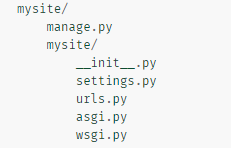
\includegraphics{figuras/311/img1.png}	 
	 \renewcommand{\arraystretch}{1.3}
	 \caption{Árbol de la carpeta \textbf{mysite}}
  \end{center}
\end{figure}
	\end{minipage}
\end{figure} 
\color{black}{}

Enumeremos estos archivos:

\begin{enumerate}
\item 
El directorio externo \textbf{mysite/root} es un contenedor para su proyecto. Su nombre no le importa a \django{}; puedes cambiarle el nombre a lo que quieras

\item 
\textbf{manage.py:} es una utilidad de línea de comandos que te permite interactuar con este proyecto de \django{} de varias maneras. Puede leer todos los detalles sobre \textit{manage.py} en \textcolor{B}{\href{https://docs.djangoproject.com/en/3.0/ref/django-admin/}{django-admin y manage.py}}.

\item 
El directorio \textbf{mysite/} interno es el paquete real de \py{} para su proyecto. Su nombre es el nombre del paquete \py{} que necesitará usar para importar cualquier cosa dentro de él (\textit{por ejemplo, mysite.urls}). 

\item
\textbf{mysite/\_\_ init\_\_.py:} un archivo vacío que le dice a Python que este directorio debe considerarse un paquete de Python. Si eres un principiante de \py{}, 
{\textcolor{B}{\href{https://docs.python.org/3/tutorial/modules.html}{lee mas sobre estos paquetes en la documentacion oficial  \py{}}}}

\item 
\textbf{mysite/settings.py:}  configuración para este proyecto de \django{}. La configuración de \django{} le dirá todo sobre cómo funciona la configuración ({\textcolor{B}{\href{https://docs.djangoproject.com/en/3.0/topics/settings/}{django settings}}}).

\item 
\textbf{mysite/urls.py:} las declaraciones de URL para este proyecto de \django{}; una "tabla de contenido" de su sitio impulsado por Django. Puede leer más sobre las URL en el
{\textcolor{B}{\href{https://docs.djangoproject.com/en/3.0/topics/http/urls/}{despachador de URL}}}.

\item 
\textbf{mysite/asgi.py:} Un punto de entrada para servidores web compatibles con ASGI para servir su proyecto. Consulte 
{\textcolor{B}{\href{https://docs.djangoproject.com/en/3.0/howto/deployment/asgi/}{Cómo implementar con ASGI}}} para obtener más detalles.

\item 
\textbf{mysite/wsgi.py:} 
Un punto de entrada para servidores web compatibles con WSGI para servir su proyecto. 
 Consulte {\textcolor{B}{\href{https://docs.djangoproject.com/en/3.0/howto/deployment/wsgi/}{Cómo implementar con WSGI}}} para obtener más detalles.

\end{enumerate}

\subsubsection{El servidor de desarrollo}

Verifiquemos que su proyecto \django{} funciona. Cambie al directorio externo de \textbf{mysite}, si aún no lo ha hecho, y ejecute el siguiente comando:
$$
\fbox{\$ python manage.py runserver}
$$
Luego, deberías ver sobre la linea de comandos, algo similar a lo que aparece en la siguiente imagen:

\begin{figure}[H]
  \begin{center}
  	 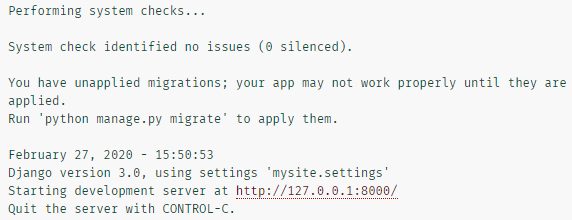
\includegraphics{figuras/312/img1.png}	 
	 \renewcommand{\arraystretch}{1.3}
	 \caption{Inicio del servidor de django sobre la linea de comandos}
  \end{center}
\end{figure}

Has iniciado el servidor de desarrollo \django{}, un servidor web ligero escrito exclusivamente en \py{}. Hemos incluido esto con \django{} para que pueda desarrollar las cosas rápidamente, sin tener que lidiar con la configuración de un servidor de producción, como \textbf{Apache}, hasta que esté listo para la producción.


Ahora es un buen momento para tener en cuenta que no debe usar este servidor en nada parecido a un entorno de producción. Está destinado solo para su uso durante el desarrollo. 

Ahora que el servidor se está ejecutando, visite $http://127.0.0.1:8000/$ con su navegador web. Verás un \textbf{"¡Felicitaciones!"} sobre la página y con un cohete despegando. Si es asi entonces ¡Funcionó!.

\begin{table}[H]
	%\renewcommand{\arraystretch}{1.3}	
	\begin{tabular}{||c||}
	\hline \\
	\begin{Large}
	\textbf{\textit{Cambiando el puerto}}
	\end{Large}
	\\\\
			De manera predeterminada, el comando runserver inicia el servidor de desarrollo en la IP interna en el puerto 8000.\\
Si desea cambiar el puerto del servidor, páselo como un argumento de línea de comandos.\\Por ejemplo, este comando inicia el servidor en el puerto 8080:
\\\\
$$\fbox{\$ python manage.py runserver 8080}$$
\\\\
Si desea cambiar la IP del servidor, páselo junto con el puerto.\\ Por ejemplo, para escuchar todas las IP públicas disponibles\\ (lo cual es útil si está ejecutando Vagrant o desea mostrar su trabajo en otras computadoras en la red), use:
\\\\$$\fbox{\$ python manage.py runserver 0:8000}$$
\\\\

0 es un atajo para 0.0.0.0. Los documentos completos para el servidor de desarrollo se pueden encontrar en \\la referencia del servidor de ejecución.
	\\ \hline 	
			\end{tabular}
		\end{table}		
		
\begin{table}[H]
	%\renewcommand{\arraystretch}{1.3}	
	\begin{tabular}{||c||}
	\hline \\
	\begin{Large}
	\textbf{\textit{Reinicio automático del servidor}}
	\end{Large}
	\\\\		
El servidor de desarrollo vuelve a cargar automáticamente el código \py{} para cada solicitud según sea necesario.\\ No necesita reiniciar el servidor para que los cambios de código surtan efecto.\\ Sin embargo, algunas acciones como agregar archivos no activan un reinicio, por lo que deberá reiniciar el servidor \\en estos casos.
\\ \hline 	
			\end{tabular}
		\end{table}		

\subsubsection{Creando la aplicación de encuestas (polls)}
Una vez que su entorno de proyecto esta listo y configurado, estamos listos para empezar a trabajar.


Cada aplicación que escribe en \django{} consiste en un paquete de \py{} que sigue una determinada convención. \django{} viene con una utilidad que genera automáticamente la estructura básica de directorios de una aplicación, por lo que puede centrarse en escribir código en lugar de crear directorios.

\begin{table}[H]
	%\renewcommand{\arraystretch}{1.3}	
	\begin{tabular}{||c||}
	\hline \\
	\begin{Large}
	\textbf{\textit{Proyectos Vs Aplicaciones}}
	\end{Large}
	\\\\		
¿Cuál es la diferencia entre un proyecto y una aplicación?\\ Una aplicación es una aplicación web que hace algo, por ejemplo, un sistema de registro web, una base de datos de\\ registros públicos o una pequeña aplicación de encuestas.\\ Un proyecto es una colección de configuraciones y aplicaciones para un sitio web en particular. \\Un proyecto puede contener múltiples aplicaciones.\\ Una aplicación puede estar en múltiples proyectos.
\\ \hline 	
			\end{tabular}
		\end{table}		

Sus aplicaciones pueden vivir en cualquier lugar de su
{\textcolor{B}{\href{https://docs.python.org/3/tutorial/modules.htm}{ruta de Python}}}. En este tutorial, crearemos nuestra aplicación de encuestas justo al lado de su archivo \textit{manage.py} para que pueda importarse como su propio módulo de nivel superior, en lugar de un submódulo de \textit{mysite}.

Para crear su aplicación, asegúrese de estar en el mismo directorio que \textit{manage.py} y escriba este comando:

$$\fbox{\$ python manage.py startapp polls}$$

Eso creará un directorio de encuestas, que se presenta así:

\begin{figure}[H]
  \begin{center}
  	 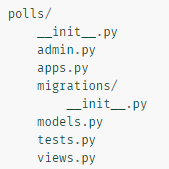
\includegraphics{figuras/313/img1.png}	 
	 \renewcommand{\arraystretch}{1.3}
	 \caption{directorio de encuestas}
  \end{center}
\end{figure}


Esta estructura de directorios albergará la aplicación de la encuesta.

\subsubsection{Escribiendo la primer vista (view)}

Escribamos la primera vista. Abra el archivo \textbf{polls/views.py} y coloque el siguiente código de \py{}:

\begin{figure}[H]
  \begin{center}
  	 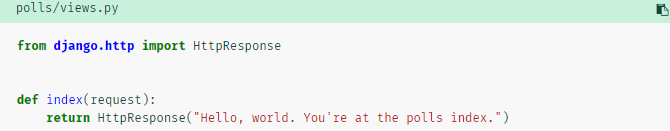
\includegraphics{figuras/314/img1.png}	 
	 \renewcommand{\arraystretch}{1.3}
	 \caption{Código \py{} de la primer vista}
  \end{center}
\end{figure}


Esta es la vista más simple posible en \django{}. Para llamar a la vista, necesitamos asignarla a una \textbf{URL}, y para esto necesitamos una \textbf{URLconf}.

Para crear una \textbf{URLconf} en el directorio de encuestas, cree un archivo llamado \textit{urls.py}. Su directorio de aplicaciones ahora debería verse como en la \textit{figura 5}
Donde en el archivo \textit{urls.py} ubicado en \textit{polls} se incluirá el código quedando este como el código de la \textit{figura 5}.

\begin{figure}[H]
  \begin{center}
  	 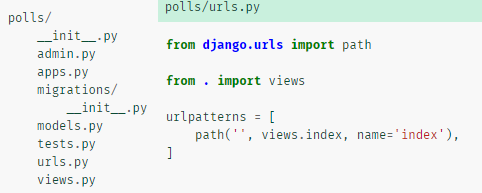
\includegraphics{figuras/314/img2.png}	 
	 \renewcommand{\arraystretch}{1.3}
	 \caption{Modificacion del directorio polls y agregado del codigo sobre el \textit{urls.py}}
  \end{center}
\end{figure}

El siguiente paso es apuntar la \textbf{URLconf} raíz al módulo \textit{polls.urls}. En \textbf{mysite/urls.py}, agregue una importación para \textcolor{G}{django.urls.include} e inserte un \textcolor{B}{\textit{include}}() en la lista \textit{urlpatterns}, Debe quedar como en la \textit{figura 6}.

\begin{figure}[H]
  \begin{center}
  	 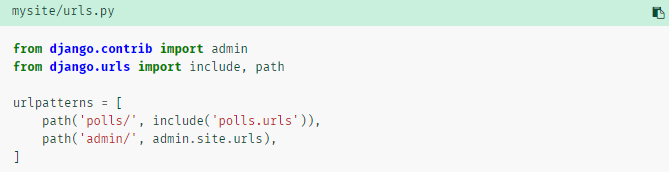
\includegraphics{figuras/314/img3.png}	 
	 \renewcommand{\arraystretch}{1.3}
	 \caption{Modificacion del codigo sobre el \textit{urls.py} del proyecto}
  \end{center}
\end{figure}

La función {\href{https://docs.djangoproject.com/en/3.0/ref/urls/#django.urls.include}{\textcolor{B}{\textit{include}}()}} permite hacer referencia a otros \textbf{URLconfs}. Cada vez que \django{} se encuentra con {\href{https://docs.djangoproject.com/en/3.0/ref/urls/#django.urls.include}{\textcolor{B}{\textit{include}}()}}, corta cualquier parte de la \textbf{URL} que coincida con ese punto y envía la cadena restante a la \textbf{URLconf} incluida para su posterior procesamiento.


La idea detrás de {\href{https://docs.djangoproject.com/en/3.0/ref/urls/#django.urls.include}{\textcolor{B}{\textit{include}}()}} es facilitar la conexión y reproducción de \textbf{URL}. Como las encuestas están en su propia \textbf{URLconf} (\textbf{polls/urls.py}), se pueden colocar debajo de \textit{/polls/}, o debajo de \textit{/fun\_ polls/}, o debajo de \textit{/content/polls/}, o cualquier otra ruta raíz, y la aplicación seguirá funcionando.

\begin{table}[H]
	%\renewcommand{\arraystretch}{1.3}	
	\begin{tabular}{||c||}
	\hline \\
	\begin{Large}
	\textbf{\textit{Cuando usamos include()}}
	\end{Large}
	\\\\		
Siempre debe usar {\href{https://docs.djangoproject.com/en/3.0/ref/urls/#django.urls.include}{\textcolor{B}{\textit{include}}()}} cuando incluya otros patrones de \textbf{URL}. \textcolor{G}{admin.site.urls} es la única excepción a esto.
\\ \hline 	
			\end{tabular}
		\end{table}		


Ahora ha conectado una vista de índice en la \textbf{URLconf}. Verifique que esté funcionando con el siguiente comando:
$$\fbox{\$ python manage.py runserver}$$


Vaya a \textit{http://localhost:8000/polls/} en su navegador, y debería ver el texto \textit{"Hello, world. You're at the polls index"}, que definiste en la vista de índice.

\begin{table}[H]
	%\renewcommand{\arraystretch}{1.3}	
	\begin{tabular}{||c||}
	\hline \\
	\begin{Large}
	\textbf{\textit{Te aparece \textbf{Page Not Found?}}}
	\end{Large}
	\\\\		
Si recibe una página de error aquí, verifique que vaya a \textit{http://localhost:8000/polls/} y no \textit{http://localhost:8000/}.
\\\\ \hline 	
			\end{tabular}
		\end{table}		

La función {\href{https://docs.djangoproject.com/en/3.0/ref/urls/#django.urls.path
}{\textcolor{B}{\textit{path}}()}} recibe cuatro argumentos, dos obligatorios: ruta y vista, y dos opcionales: kwargs y nombre. En este punto, vale la pena revisar para qué sirven estos argumentos.

\begin{itemize}
\item \textbf{\textit{Argumento route del path():}}

\textit{route} es una cadena que contiene un patrón de \textbf{URL}. Al procesar una solicitud, \django{} comienza en el primer patrón en \textit{urlpatterns} y avanza por la lista, comparando la \textbf{URL} solicitada con cada patrón hasta que encuentre uno que coincida.

Los patrones no buscan parámetros \textbf{GET} y \textbf{POST}, o el nombre de dominio. \textit{Por ejemplo}, en una solicitud a \textit{https://www.example.com/myapp/}, la \textbf{URLconf} buscará \textbf{myapp/}. En una solicitud a 

\textit{https://www.example.com/myapp/?page=3}, la \textbf{URLconf} también buscará \textbf{myapp/}.

\item \textbf{\textit{Argumento view del path():}}

Cuando \django{} encuentra un patrón coincidente, llama a la función de vista especificada con un objeto {\textcolor{B}{\href{https://docs.djangoproject.com/en/3.0/ref/request-response/}{HttpRequest}}} como primer argumento y cualquier valor ``capturado" de la ruta como argumentos de palabras clave. Vamos a dar un ejemplo de esto en un momento.

\item \textbf{\textit{Argumento kwargs del path():}}

Los argumentos de palabras clave arbitrarias se pueden pasar en un diccionario a la vista de destino. No vamos a utilizar esta función de Django en el tutorial.

\item \textbf{\textit{Argumento name del path():}}


Nombrar su \textbf{URL} le permite referirse a ella sin ambigüedades desde otros lugares de \django{}, especialmente desde las plantillas. Esta poderosa característica le permite realizar cambios globales en los patrones de \textbf{URL} de su proyecto mientras solo toca un solo archivo.
\end{itemize}

\subsection{Escribiendo tu primera aplicación \django{}, parte 2}
\subsubsection{Configuración de la Base de Datos}
Ahora, abra \textbf{mysite/settings.py}. Es un módulo \py{} normal con variables de nivel de módulo que representan la configuración de \django{}.

Por defecto, la configuración usa \textbf{SQLite}. Si eres nuevo en las bases de datos, o simplemente estás interesado en probar \django{}, esta es la opción más fácil. \textbf{SQLite} está incluido en \py{}, por lo que no necesitará instalar nada más para admitir su base de datos. Sin embargo, al comenzar su primer proyecto real, es posible que desee utilizar una base de datos más escalable como \textbf{PostgreSQL}, para evitar dolores de cabeza de cambio de base de datos en el futuro.

Si desea utilizar otra base de datos, instale los enlaces de base de datos apropiados {\textcolor{B}{\href{https://docs.djangoproject.com/en/3.0/topics/install/\#database-installation}{(database bindings)}}}
 y cambie las siguientes claves en el elemento {\textcolor{B}{\href{https://docs.djangoproject.com/en/3.0/ref/settings/\#std:setting-DATABASES}{DATABASES}}} 'default' para que coincida con la configuración de conexión de su base de datos:

\begin{itemize}
\item \textcolor {B}{\href{https://docs.djangoproject.com/en/3.0/ref/settings/\#std:setting-DATABASE-ENGINE}{ENGINE}} - Puede ser: \textcolor{G}{'django.db.backends.sqlite3'}, \textcolor{G}{'django.db.backends.postgresql'}, \textcolor{G}{'django.db.backends.mysql'}, or \textcolor{G}{'django.db.backends.oracle'}. 
Otros backends también están 
\textcolor {B}{\href{https://docs.djangoproject.com/en/3.0/ref/databases/\#third-party-notes}{disponibles}}.

\item \textcolor {B}{\href{https://docs.djangoproject.com/en/3.0/ref/settings/\#std:setting-NAME}{NAME}} - 
El nombre de su base de datos. Si está utilizando \textbf{SQLite}, la base de datos será un archivo en su computadora; en ese caso, \textcolor {B}{\href{https://docs.djangoproject.com/en/3.0/ref/settings/\#std:setting-NAME}{NAME}} debe ser la ruta absoluta completa, incluido el nombre de archivo, de ese archivo. El valor predeterminado, \textcolor{G}{os.path.join (BASE\_DIR, 'db.sqlite3')}, almacenará el archivo en el directorio de su proyecto.

\end{itemize}

Si no está utilizando \textbf{SQLite} como su base de datos, se deben agregar configuraciones adicionales como \textcolor {B}{\href{https://docs.djangoproject.com/en/3.0/ref/settings/\#std:setting-USER}{USUARIO}}
, \textcolor {B}{\href{https://docs.djangoproject.com/en/3.0/ref/settings/\#std:setting-PASSWORD}{CONTRASEÑA}}
 y \textcolor {B}{\href{https://docs.djangoproject.com/en/3.0/ref/settings/\#std:setting-HOST}{HOST}}
. Para obtener más detalles, consulte la documentación de referencia para \textcolor {B}{\href{https://docs.djangoproject.com/en/3.0/ref/settings/\#std:setting-DATABASES}{BASES DE DATOS}}.

\begin{table}[H]
	%\renewcommand{\arraystretch}{1.3}	
	\begin{tabular}{||c||}
	\hline \\
	\begin{Large}
	\textbf{\textit{Para bases de datos que no sean SQLite}}
	\end{Large}
	\\\\		
Si está utilizando una base de datos además de \textbf{SQLite}, asegúrese de haber creado una base de datos\\ en este momento. Haga eso con \textcolor{G}{$"CREATE$ $DATABASE$ $database\_name;"$} dentro de la solicitud \\interactiva de su base de datos.
También asegúrese de que el usuario de la base de datos proporcionado en\\ \textbf{mysite/settings.py} tenga privilegios de "crear base de datos". Esto permite la creación automática\\ de una base de datos de prueba que será necesaria en un tutorial posterior.\\
Si está utilizando \textbf{SQLite}, no necesita crear nada de antemano; el archivo de la base de datos se creará\\ automáticamente cuando sea necesario.
\\\\ \hline 	
			\end{tabular}
		\end{table}		


Mientras editas \textbf{mysite/settings.py}, configura {\textcolor{B}{\href{https://docs.djangoproject.com/en/3.0/ref/settings/\#std:setting-TIME\_ZONE}{TIME\_ZONE}}}
 en su zona horaria.

Además, tenga en cuenta la configuración {\textcolor{B}{\href{https://docs.djangoproject.com/en/3.0/ref/settings/\#std:setting-INSTALLED\_APPS}{INSTALLED\_APPS}}}
 en la parte superior del archivo. Esta contiene los nombres de todas las aplicaciones de \django{} que se activan en esta instancia de \django{}. Las aplicaciones se pueden usar en múltiples proyectos, y puede empaquetarlas y distribuirlas para que otras personas las usen en sus proyectos.


Por defecto, {\href{https://docs.djangoproject.com/en/3.0/ref/settings/\#std:setting-INSTALLED\_APPS}{INSTALLED\_APPS}} contiene las siguientes aplicaciones, las cuales se instalan al instalar \django{} 

\begin{itemize}
%{\href{}{\textcolor{B}{}}}
%1
\item {\href{https://docs.djangoproject.com/en/3.0/ref/contrib/admin/\#module-django.contrib.admin}{\textcolor{B}{django.contrib.admin}}} – Sitio de administración.
%2
\item {\href{https://docs.djangoproject.com/en/3.0/topics/auth/\#module-django.contrib.auth}{\textcolor{B}{django.contrib.auth}}} – Sistema de autenticación.
%3
\item {\href{https://docs.djangoproject.com/en/3.0/ref/contrib/contenttypes/\#module-django.contrib.contenttypes}{\textcolor{B}{django.contrib.contenttypes}}} – 
Un marco para los tipos de contenido.
%4
\item {\href{https://docs.djangoproject.com/en/3.0/topics/http/sessions/\#module-django.contrib.sessions}{\textcolor{B}{django.contrib.sessions}}} – framework (marco) de sesiones.
%5
\item {\href{https://docs.djangoproject.com/en/3.0/ref/contrib/messages/\#module-django.contrib.messages}{\textcolor{B}{django.contrib.messages}}} – framework (marco) de mensajes.
%6
\item {\href{https://docs.djangoproject.com/en/3.0/ref/contrib/staticfiles/\#module-django.contrib.staticfiles}{\textcolor	{B}{django.contrib.staticfiles}}} – 
Un marco para administrar archivos estáticos.

\end{itemize}

Estas aplicaciones se incluyen por defecto como una conveniencia para casos específicos.

Sin embargo, algunas de estas aplicaciones utilizan al menos una tabla de base de datos, por lo que debemos crear las tablas en la base de datos antes de poder usarlas. Para hacer eso, ejecuta el siguiente comando:

$$\fbox{\$ python manage.py migrate}$$

El comando migrate analiza la configuración {\href{https://docs.djangoproject.com/en/3.0/ref/settings/\#std:setting-INSTALLED\_APPS}{\textcolor{B}{INSTALLED\_APPS}}} y crea las tablas de base de datos necesarias de acuerdo con la configuración de la base de datos en su archivo \textbf{mysite/settings.py} y las migraciones de la base de datos que se envían con la aplicación (las cubriremos más adelante). Verá un mensaje para cada migración que aplique. Si está interesado, ejecute el cliente de línea de comandos para su base de datos y escriba \textbackslash dt (PostgreSQL), MOSTRAR TABLAS; (MariaDB, MySQL), .schema (SQLite) o SELECT TABLE\_NAME FROM USER\_TABLES; (Oracle) para mostrar las tablas que Django creó.

\begin{table}[H]
	%\renewcommand{\arraystretch}{1.3}	
	\begin{tabular}{||c||}
	\hline \\
	\begin{Large}
	\textbf{\textit{Para los minimalistas}}
	\end{Large}
	\\\\		
Como dijimos anteriormente, las aplicaciones predeterminadas se incluyen para el caso común, pero no todos\\ las necesitan. Si no necesita ninguno o todos ellos, no dude en comentar o eliminar las líneas apropiadas de\\ {\href{https://docs.djangoproject.com/en/3.0/ref/settings/\#std:setting-INSTALLED\_APPS}{\textcolor{B}{INSTALLED\_APPS}}} antes de ejecutar la {\href{https://docs.djangoproject.com/en/3.0/ref/django-admin/\#django-admin-migrate}{\textcolor{B}{migración}}}
.\\ El comando {\href{https://docs.djangoproject.com/en/3.0/ref/django-admin/\#django-admin-migrate}{\textcolor{B}{migrate}}}
 solo ejecutará migraciones para aplicaciones en {\href{https://docs.djangoproject.com/en/3.0/ref/settings/\#std:setting-INSTALLED\_APPS}{\textcolor{B}{INSTALLED\_APPS}}}.
\\\\ \hline 	
			\end{tabular}
		\end{table}		

\subsubsection{Creando un Modelo}

\begin{table}[H]
	%\renewcommand{\arraystretch}{1.3}	
	\begin{tabular}{||c||}
	\hline \\
	\begin{Large}
	\textbf{\textit{Filosofia}}
	\end{Large}
	\\\\		
Un modelo es la fuente única y definitiva de verdad sobre sus datos. Contiene los campos y \\comportamientos esenciales de los datos que está almacenando.\\ \django{} sigue el principio DRY ({\href{https://docs.djangoproject.com/en/3.0/misc/design-philosophies/\#dry}{\textcolor{B}{DRY principle}}}).\\ El objetivo es definir su modelo de datos en un lugar y derivar automáticamente cosas de él.\\

Esto incluye las migraciones, a diferencia de \textbf{Ruby On Rails}, por ejemplo, las migraciones\\ se derivan completamente de su archivo de modelos, y son esencialmente un historial que\\ \django{} puede recorrer para actualizar su esquema de base de datos para que coincida con sus\\ modelos actuales.
\\\\ \hline 	
			\end{tabular}
		\end{table}		

En nuestra aplicación de encuestas, crearemos dos modelos: Pregunta (Question) y Elección (Choice). 

\begin{figure}[H]
	\begin{center}
		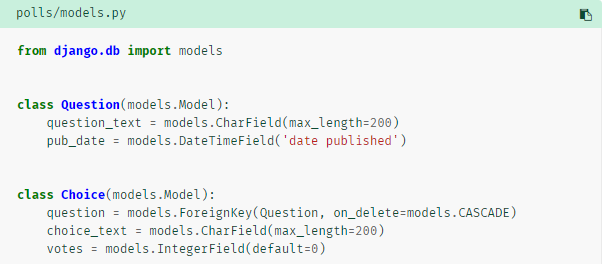
\includegraphics[scale=0.7]{figuras/322/img1.png}
		\renewcommand{\arraystretch}{1.3}
		\caption{Codigo de los modelos \textbf{Question} y \textbf{Choice}}
	\end{center}
\end{figure}
Una Question tiene una pregunta y una fecha de publicación. Una opción tiene dos campos: el texto de la opción y un conteo de votos. Cada opción está asociada con una pregunta.

Estos conceptos están representados por las clases de \py. Edite el archivo \textbf{polls/models.py} para que se vea como en la \textit{figura 7}.

Aquí, cada modelo está representado por una clase que subclasifica {\href{https://docs.djangoproject.com/en/3.0/ref/models/instances/\#django.db.models.Model}{\textcolor{B}{django.db.models.Model}}}	. Cada modelo tiene una serie de variables de clase, cada una de las cuales representa un campo de base de datos en el modelo.

Cada campo está representado por una instancia de clase {\href{https://docs.djangoproject.com/en/3.0/ref/models/fields/\#django.db.models.Field}{\textcolor{B}{Campo}}}, por ejemplo, {\href{https://docs.djangoproject.com/en/3.0/ref/models/fields/\#django.db.models.CharField}{\textcolor{B}{CharField}}} para campos de caracteres y {\href{https://docs.djangoproject.com/en/3.0/ref/models/fields/\#django.db.models.DateTimeField}{\textcolor{B}{DateTimeField}}}
 para fechas y horas. Esto le dice a \django{} qué tipo de datos contiene cada campo.

El nombre de cada instancia de campo (por ejemplo, question\_text o pub\_date) es el nombre del campo, en formato amigable para la máquina. Utilizará este valor en su código de \py{}, y su base de datos lo usará como el nombre de la columna

Puede usar un primer argumento posicional opcional del campo para designar un nombre que sea legible por humanos. Eso se usa en un par de partes introspectivas de \django{}, y también sirve como documentación. Si no se proporciona este campo, \django{} usará el nombre legible por la máquina. En este ejemplo, solo hemos definido un nombre legible para humanos para \textcolor{G}{Question.pub\_date}. Para todos los demás campos en este modelo, el nombre del campo legible por la máquina será suficiente como su nombre legible por humanos.

Algunas clases de campo tienen argumentos requeridos. {\href{https://docs.djangoproject.com/en/3.0/ref/models/fields/\#django.db.models.CharField}{\textcolor{B}{CharField}}}, por ejemplo, requiere que le des una \textbf{longitud máxima} ({\href{https://docs.djangoproject.com/en/3.0/ref/models/fields/\#django.db.models.CharField.max_length}{\textcolor{B}{max\_length}}}). Eso se usa no solo en el esquema de la base de datos, sino también en la validación.

Un campo también puede tener varios argumentos opcionales; en este caso, hemos establecido el valor predeterminado ({\href{https://docs.djangoproject.com/en/3.0/ref/models/fields/\#django.db.models.Field.default}{\textcolor{B}{default}}}) de votos en 0.

Finalmente, tenga en cuenta que se define una relación, usando {\href{https://docs.djangoproject.com/en/3.0/ref/models/fields/#django.db.models.ForeignKey}{\textcolor{B}{ForeingKey}}}
. Eso le dice a \django{} que cada Elección está relacionada con una sola Pregunta. \django{} admite todas las relaciones de base de datos comunes: muchas a una, muchas a muchas y una a una.


\subsubsection{Modelos de Activación}

Ese pequeño fragmento de código del modelo le da a \django{} bastante información. Con él, \django{} es capaz de:
\begin{itemize}
\item 
Crear un esquema de base de datos (sentencias CREATE TABLE) para esta aplicación.
\item
Crear una \textbf{API} de acceso a la base de datos de \py{} para acceder a los objetos \textbf{Question} y \textbf{Choice}.
\end{itemize}

Pero primero debemos decirle a nuestro proyecto \textit{que la aplicación de encuestas está instalada}.


\begin{table}[H]
	%\renewcommand{\arraystretch}{1.3}	
	\begin{tabular}{||c||}
	\hline \\
	\begin{Large}
	\textbf{\textit{Filosofia}}
	\end{Large}
	\\\\		
Las aplicaciones de \django{} son "conectables": puede usar una aplicación en varios proyectos y puede\\ distribuir aplicaciones,ya que no tienen que estar vinculadas a una determinada instalación de \django{}.
\\\\ \hline 	
			\end{tabular}
		\end{table}		


Para incluir la aplicación en nuestro proyecto, necesitamos agregar una referencia a su clase de configuración en la configuración {\href{https://docs.djangoproject.com/en/3.0/ref/settings/\#std:setting-INSTALLED\_APPS}{\textcolor{B}{INSTALLED\_APPS}}}. La clase \textcolor{G}{PollsConfig} está en el archivo \textbf{polls/apps.py}, por lo que su ruta punteada es \textcolor{G}{'polls.apps.PollsConfig'}. Hay que editar el archivo mysite/settings.py y agreguar esa ruta punteada a la configuración {\href{https://docs.djangoproject.com/en/3.0/ref/settings/\#std:setting-INSTALLED\_APPS}{\textcolor{B}{INSTALLED\_APPS}}}. Se verá así:

\begin{figure}[H]
	\begin{center}
		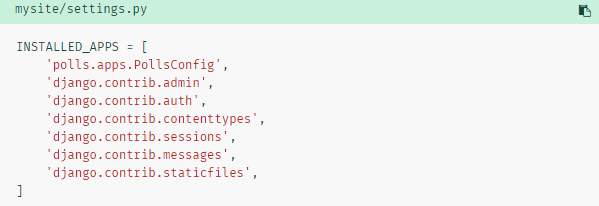
\includegraphics[scale=0.9]{figuras/323/img1.png}
		\renewcommand{\arraystretch}{1.3}
		\caption{Instalación de la aplicación polls en el \textcolor{G}{settings.py} del proyecto }
	\end{center}
\end{figure}


Listo, \django{} con esto ya sabe incluir la aplicación de encuestas. Ahora, debemos aplicar migraciones, lo cual se hace con el comando:

$$\fbox{\$ python manage.py makemigrations polls}$$

Luego, en la terminal vas a ver algo similar a:

\begin{figure}[H]
\begin{center}
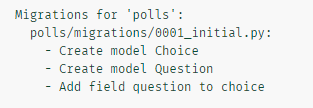
\includegraphics[scale=1]{figuras/323/img2.png}
\renewcommand{\arraystretch}{1.3}
\caption{Terminal con un makemigrations satisfactorio}
\end{center}
\end{figure}


Al correr \textit{makemigrations}, le estás diciendo a Django que has realizado algunos cambios en tus modelos (En este caso, agregaste modelos al \textbf{models.py}) y que queremos que esos cambios sean almacenados como migraciones.


Las migraciones es la forma en la cual \django{} almacena los cambios en sus modelos (y, por lo tanto, en el esquema de su base de datos): estos son archivos en el disco. Podemos leer las migraciones si queremos; en este caso son las encuestas de \textbf{polls/migrations/0001\_initial.py}. No se preocupe, no se espera que los lea cada vez que Django hace uno, pero están diseñados para ser editados por humanos en caso de que desee modificar manualmente cómo \django{} cambia las cosas.


Hay un comando que ejecutará las migraciones por usted y administrará el esquema de su base de datos automáticamente, este es el comando \textit{migrate}, y lo veremos en un momento, pero primero, veamos qué \textbf{SQL} ejecutará esa migración. El comando \textit{sqlmigrate} toma nombres de migración y devuelve su SQL:

$$\fbox{\$ python manage.py sqlmigrate polls 0001}$$

Vas a ver algo similar a esto, quizas en otro formato pero con el mismo contenido:


\begin{figure}[H]
\begin{center}
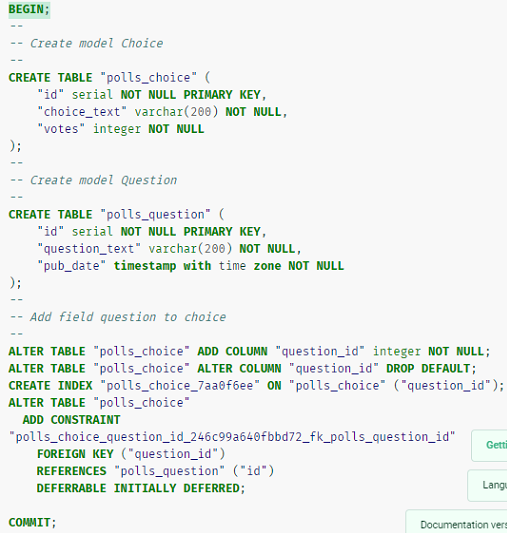
\includegraphics[scale=0.7]{figuras/323/img3.png}
\renewcommand{\arraystretch}{1.3}
\caption{python manage.py sqlmigrate polls 0001}
\end{center}
\end{figure}

Notemos que:

\begin{itemize}
\item 
El resultado exacto variará según la base de datos que esté utilizando. El ejemplo anterior se genera para PostgreSQL.

\item
Los nombres de las tablas se generan automáticamente combinando el nombre de la aplicación (encuestas) y el nombre en minúsculas del modelo: pregunta y elección. (Puede anular este comportamiento).

\item 
Las claves primarias (ID) se agregan automáticamente. (También puede anular esto).

\item 
Por convención, \django{} agrega "\_id" al nombre del campo de clave externa. (Sí, también puedes sobrescribirlo).

\item 
La relación de clave externa se hace explícita por una restricción FOREIGN KEY. No se preocupe por las partes DEFERRABLES; esto le dice a PostgreSQL que no aplique la clave foránea hasta el final de la transacción

\item 
Se adapta a la base de datos que está utilizando, por lo que los tipos de campo específicos de la base de datos como auto\_increment (MySQL), serial (PostgreSQL) o autoincrement de clave primaria entera (SQLite) se manejan automáticamente. Lo mismo ocurre con las citas de los nombres de campo, por ejemplo, con comillas dobles o comillas simples.

\item 
El comando \textit{sqlmigrate} no ejecuta realmente la migración en su base de datos, sino que lo imprime en la pantalla para que pueda ver lo que \textbf{SQL Django} cree que es necesario. Es útil para verificar qué hará \django{} o si tiene administradores de bases de datos que requieren \textit{scripts SQL} para dichos cambios.
\end{itemize}

Si está interesado, también puede ejecutar \textit{python manage.py check}; Esto verifica si hay algún problema en su proyecto sin hacer migraciones o tocar la base de datos.

Ahora, debemos correr el comando \textit{migrate} otra vez para crear estos modelos en las tablas de tu base de datos.

\begin{figure}[H]
\begin{center}
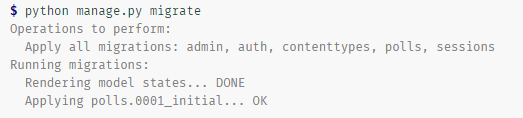
\includegraphics[scale=1]{figuras/323/img4.png}
\renewcommand{\arraystretch}{1.3}
\caption{python manage.py sqlmigrate polls 0001}
\end{center}
\end{figure}


El comando \textit{migrate} toma todas las migraciones que no se han aplicado (\django{} rastrea cuáles se aplican usando una tabla especial en su base de datos llamada \textcolor{G}{django\_migrations}) y las ejecuta en su base de datos, esencialmente, sincronizando los cambios que realizó en sus modelos con el esquema en la base de datos.

Las migraciones son muy potentes y le permiten cambiar sus modelos con el tiempo, a medida que desarrolla su proyecto, sin la necesidad de eliminar su base de datos o tablas y crear nuevas: se especializa en actualizar su base de datos en vivo, sin perder datos. Los cubriremos con más profundidad en una parte posterior del tutorial, pero por ahora, recuerde la guía de tres pasos para realizar cambios en el modelo:

\begin{itemize}
\item
Creamos/modificamos los modelos en el archivo \textit{models.py}.

\item
Luego corremos el comando \textit{python manage.py makemigrations} para crear las migraciones para esos cambios.

\item
Corremos el comando \textit{python manage.py migrate} para aplicar los cambios realizados en la base de datos.
\end{itemize}

La razón por la que existen comandos separados para realizar y aplicar migraciones es porque comprometerás las migraciones en tu sistema de control de versiones y las enviarás con tu aplicación; no solo facilitan su desarrollo, también pueden ser utilizados por otros desarrolladores y en producción.

\subsubsection{Jugando con la API}

Ahora, entremos al \textit{shell} interactivo de \py{} y juguemos con la \textbf{API} gratuita que \django{} le brinda. Para invocar el \textit{shell} de \py{}, use este comando:

$$\fbox{\$ python manage.py shell}$$


Estamos usando esto en lugar de simplemente escribir \textit{"python"}, porque \textit{manage.py} establece la variable de entorno \textcolor{G}{DJANGO\_SETTINGS\_MODULE}, que le da a \django{} la ruta de importación de \py{} a su archivo \textbf{mysite/settings.py}.

Una ves que entramos en la \textit{shell} podemos trabajar con ella realizando {\href{https://docs.djangoproject.com/en/3.0/topics/db/queries/}{\textcolor{B}{consultas}}} como se indica en la figura:
\begin{figure}[H]
\begin{center}
\renewcommand{\arraystretch}{1.3}
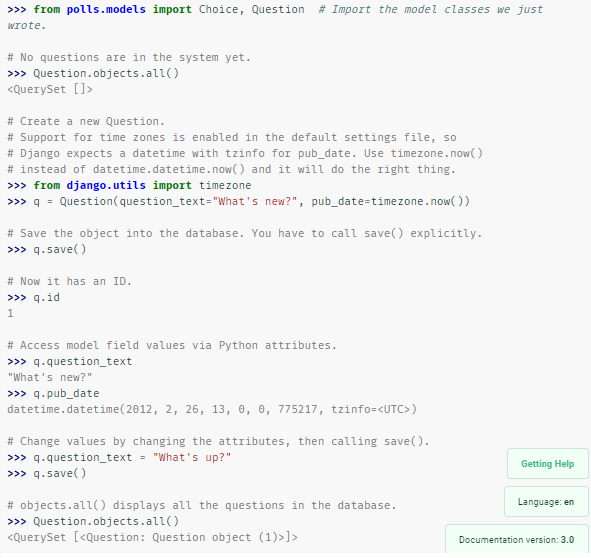
\includegraphics[scale=1.1]{figuras/324/img1.png}
\caption{Making queries}
\end{center}
\end{figure}


Ahora, vemos una cosa \textbf{$<$Question: Question object (1)$>$} no es una representación útil de este objeto. Arreglemos eso editando el modelo Question (en el archivo \textbf{polls/models.py}) y agregando un método{\href{https://docs.djangoproject.com/en/3.0/ref/models/instances/\#django.db.models.Model.\_\_str\_\_()}{\textcolor{B}{\_\_str \_\_()}}}  a los modelos \textbf{Question} y \textbf{Choice}:
\newpage
\begin{figure}[H]
\begin{center}
\renewcommand{\arraystretch}{1.3}
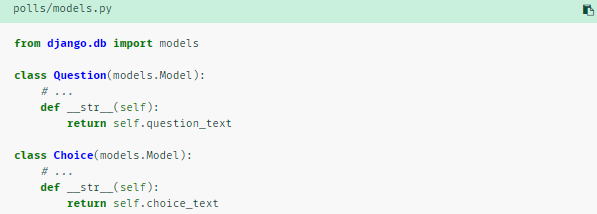
\includegraphics[scale=1]{figuras/324/img2.png}
\caption{•}
\end{center}
\end{figure}

Es importante agregar los métodos {\href{https://docs.djangoproject.com/en/3.0/ref/models/instances/\#django.db.models.Model.\_\_str\_\_()}{\textcolor{B}{\_\_str \_\_()}}} a sus modelos, no solo para su propia conveniencia al tratar con el mensaje interactivo, sino también porque las representaciones de los objetos se utilizan en todo el administrador generado automáticamente por \django{}.

Agreguemos también un método personalizado a este modelo:
\\
\begin{figure}[H]
\begin{center}
\renewcommand{\arraystretch}{1.3}
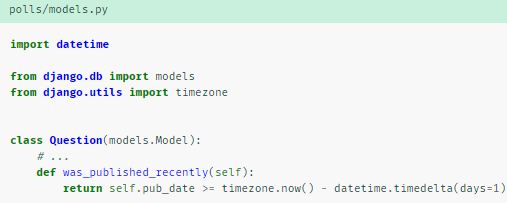
\includegraphics[scale=1]{figuras/324/img3.png}
\caption{•}
\end{center}
\end{figure}

Observe la adición de \textcolor{G}{import datetime} y de \textcolor{G}{django.utils import timezone}, para hacer referencia al módulo de fecha y hora estándar de \py{} y las utilidades relacionadas con la zona horaria de \django{} en \textcolor{G}{django.utils.timezone}, respectivamente. Si no está familiarizado con el manejo de zona horaria en \py{}, puede obtener más información en los documentos de soporte de zona horaria.


Guarde estos cambios e inicie un nuevo \textit{shell} interactivo de \py{} ejecutando nuevamente \textit{python manage.py shell}:

\begin{figure}[H]
\begin{center}
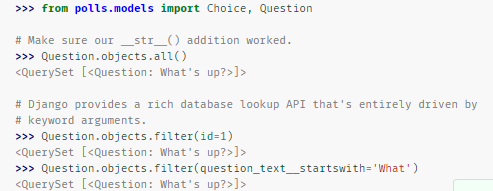
\includegraphics[scale=1]{figuras/324/img4.png}
\end{center}
\end{figure}
\begin{figure}[H]
\begin{center}
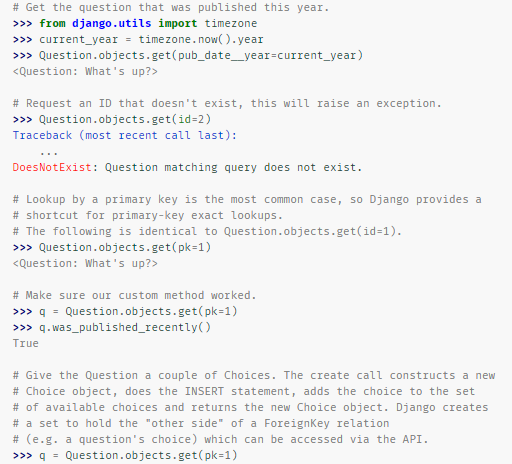
\includegraphics[scale=1]{figuras/324/img5.png}
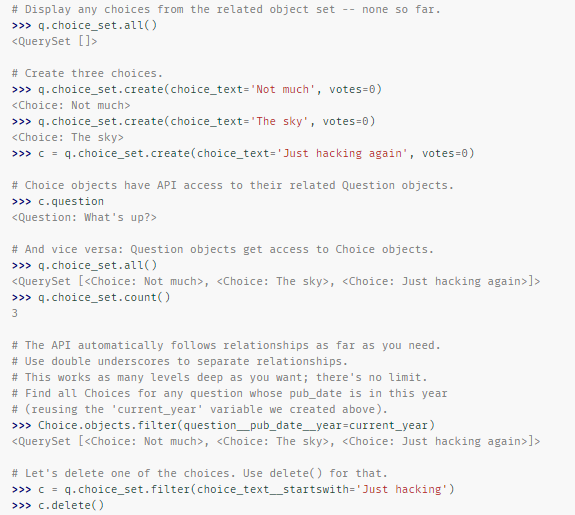
\includegraphics[scale=0.9]{figuras/324/img6.png}
\end{center}
\end{figure}

Para obtener más información sobre las relaciones del modelo, consulte Acceso a objetos relacionados ({\href{https://docs.djangoproject.com/en/3.0/ref/models/relations/}{\textcolor{B}{Accessing related objects}}}
). Para obtener más información sobre cómo utilizar guiones bajos dobles para realizar búsquedas de campo a través de la API, consulte las búsquedas de campo ({\href{https://docs.djangoproject.com/en/3.0/topics/db/queries/\#field-lookups-intro}{\textcolor{B}{field lookups}}}
). Para obtener detalles completos sobre la API de base de datos, consulte nuestra referencia de API de base de datos ({\href{https://docs.djangoproject.com/en/3.0/topics/db/queries/}{\textcolor{B}{Database API reference}}}).

\subsubsection{Introducción al administrador de \django{}}

\begin{table}[H]
	%\renewcommand{\arraystretch}{1.3}	
	\begin{tabular}{||c||}
	\hline \\
	\begin{Large}
	\textbf{\textit{Filosofia}}
	\end{Large}
	\\\\		
Generar sitios de administración para que su personal o clientes agreguen, cambien y eliminen\\ contenido es un trabajo tedioso que no requiere mucha creatividad. Por esa razón, \django{}\\ automatiza por completo la creación de interfaces de administración para modelos.\\

\django{} fue escrito en un entorno de redacción, con una separación muy clara entre los \\ ``editores de contenido'' y el sitio ``público''.\\ Los administradores del sitio usan el sistema para agregar noticias, \\ eventos, resultados deportivos, etc., y ese contenido se muestra en el sitio público.\\ \django{} resuelve el problema de crear una interfaz unificada para que los administradores \\ del sitio editen contenido.\\

El administrador no está destinado a ser utilizado por los visitantes del sitio.\\ Es para los administradores del sitio.
\\\\ \hline 	
			\end{tabular}
		\end{table}		

\subsubsection*{Creando un usuario administrador}

Crear un usuario administrador Primero, necesitaremos crear un usuario que pueda iniciar sesión en el sitio de administración. Ejecute el siguiente comando:

$$\fbox{\$ python manage.py createsuperuser}$$

Al correr este comando nos pedira una serie de datos, como el nombre del \textit{usuario}, \textit{nuestro mail} y una \textit{contraseña}.

\subsubsection*{Corremos el servidor de desarrollo}
El administrador de \django{} ya viene activado por defecto. 
Primero debemos correr el servidor una vez creado el administrador:

$$\fbox{\$ python manage.py runserver}$$


Ahora, abra un navegador web y vaya a \textbf{/ admin /} en su dominio local, por ejemplo, \textbf{http://127.0.0.1:8000/admin/}. Debería ver la pantalla de inicio de sesión del administrador:

\begin{figure}[H]
\begin{center}
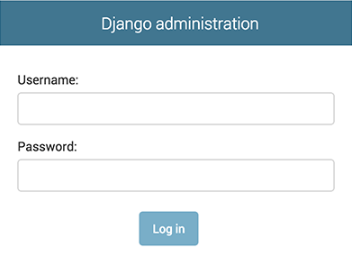
\includegraphics[scale=0.9]{figuras/325/img1.png}
\caption{Login del administrador}
\end{center}
\end{figure}


Dado que la traducción ({\href{https://docs.djangoproject.com/en/3.0/topics/i18n/translation/}{\textcolor{B}{traslation}}}
) está activada de manera predeterminada, la pantalla de inicio de sesión puede mostrarse en su propio idioma, según la configuración de su navegador y si \django{} tiene una traducción para este idioma.

\subsubsection*{El sitio de administración}

Ahora, intente iniciar sesión con la cuenta de \textit{superusuario} que creó en el paso anterior. Debería ver la página de índice de administración de \django{}:

\begin{figure}[H]
\begin{center}
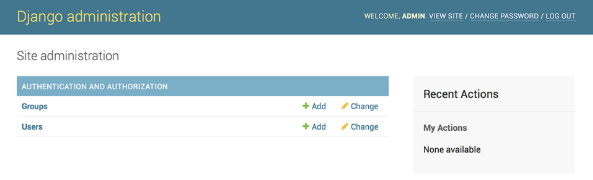
\includegraphics[scale=0.9]{figuras/325/img2.png}
\caption{Login del administrador}
\end{center}
\end{figure}


Debería ver algunos tipos de contenido editable: grupos y usuarios. Estos los proporciona {\href{https://docs.djangoproject.com/en/3.0/topics/auth/#module-django.contrib.auth}{\textcolor{B}{django.contrib.auth}}}
, el cual es el \textit{marco de autenticación} enviado por \django{}.

\subsubsection*{Hacer que la aplicación de la aplicacion sea modificable en el administrador}

¿Pero dónde está nuestra aplicación de encuestas? No se muestra en la página de índice de administrador.

Solo una cosa más que hacer: necesitamos decirle al administrador que los objetos de Pregunta tienen una interfaz de administrador. Para hacer esto, abra el archivo \textbf{polls/admin.py} y edítelo para que se vea así:

\begin{figure}[H]
\begin{center}
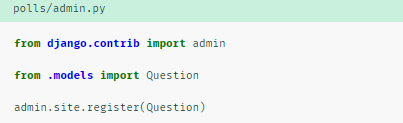
\includegraphics[scale=0.9]{figuras/325/img3.png}
\caption{Login del administrador}
\end{center}
\end{figure}

\subsubsection*{Explore la funcionalidad de administración gratuita}


Ahora que hemos registrado el modelo \textbf{Question}, \django{} sabe que debería mostrarse en la página de índice de administración:

\begin{figure}[H]
\begin{center}
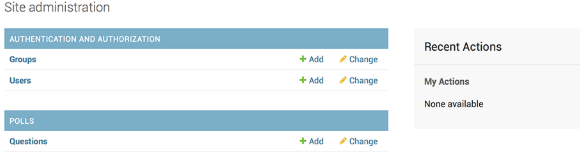
\includegraphics[scale=0.9]{figuras/325/img4.png}
\caption{Login del administrador}
\end{center}
\end{figure}


Haga clic en \textbf{``Question''}. Ahora está en la página de "lista de cambios" para Question. Esta página muestra todas las preguntas en la base de datos y le permite elegir una para cambiarla. Ahí está el "¿Qué pasa?" pregunta que creamos anteriormente:

\begin{figure}[H]
\begin{center}
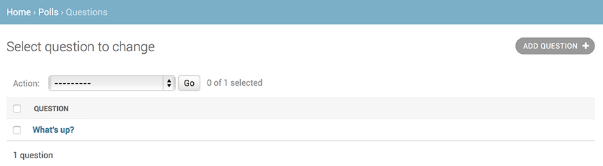
\includegraphics[scale=0.9]{figuras/325/img5.png}
\caption{Login del administrador}
\end{center}
\end{figure}


Haz clic en "¿Qué pasa?" pregunta para editarlo:

\begin{figure}[H]
\begin{center}
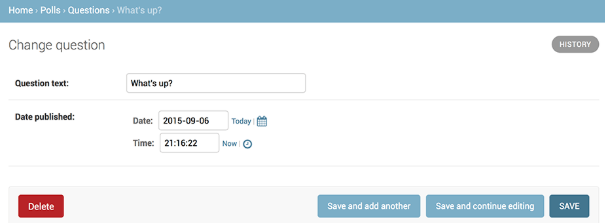
\includegraphics[scale=0.9]{figuras/325/img6.png}
\caption{Modificando la Question}
\end{center}
\end{figure}

Acá debemos tener en cuenta que:

\begin{itemize}
\item 
El formulario se genera automáticamente a partir del modelo de Pregunta.

\item 
Los diferentes tipos de campo de modelo ({\href{https://docs.djangoproject.com/en/3.0/ref/models/fields/\#django.db.models.DateTimeField}{\textcolor{B}{DateTimeField}}}, {\href{https://docs.djangoproject.com/en/3.0/ref/models/fields/\#django.db.models.CharField}{\textcolor{B}{CharField}}}
) corresponden al \textit{widget} de entrada \textbf{HTML} apropiado. Cada tipo de campo sabe cómo mostrarse en el administrador de \django{}.

\item
Cada {\href{https://docs.djangoproject.com/en/3.0/ref/models/fields/\#django.db.models.DateTimeField}{\textcolor{B}{DateTimeField}}} obtiene accesos directos de \textbf{JavaScript} gratuitos. Las fechas obtienen un acceso directo "Hoy" y una ventana emergente de calendario, y las horas obtienen un acceso directo "Ahora" y una ventana emergente conveniente que enumera las horas comúnmente ingresadas.


La parte inferior de la página le ofrece un par de opciones:

\item
Guardar: guarda los cambios y vuelve a la página de lista de cambios para este tipo de objeto.

\item
Guardar y continuar editando: guarda los cambios y vuelve a cargar la página de administración para este objeto.

\item
Guardar y agregar otro: guarda los cambios y carga un nuevo formulario en blanco para este tipo de objeto

\item
Eliminar: muestra una página de confirmación de eliminación

\end{itemize}


Si el valor de "Fecha de publicación" no coincide con la hora en que creó la pregunta en el Tutorial 1, probablemente significa que olvidó establecer el valor correcto para la configuración {\href{https://docs.djangoproject.com/en/3.0/ref/settings/\#std:setting-TIME\_ZONE}{\textcolor{B}{TIME\_ZONE}}}. Cámbielo, vuelva a cargar la página y verifique que aparezca el valor correcto.

Cambie la "Fecha de publicación" haciendo clic en los accesos directos "Hoy" y "Ahora". Luego haga clic en "Guardar y continuar editando". Luego haga clic en "Historial" en la esquina superior derecha. Verá una página que enumera todos los cambios realizados en este objeto a través del administrador de Django, con la marca de tiempo y el nombre de usuario de la persona que realizó el cambio:

\begin{figure}[H]
\begin{center}
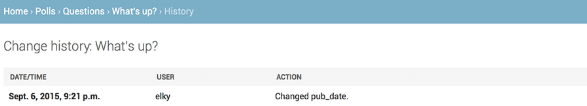
\includegraphics[scale=0.9]{figuras/325/img7.png}
\caption{Modificando la Question}
\end{center}
\end{figure}

Cuando se sienta cómodo con la API de modelos y se haya familiarizado con el sitio de administración, lea la {\href{https://docs.djangoproject.com/en/3.0/intro/tutorial03/}{\textcolor{B}{parte 3}}}  de este tutorial para obtener información sobre cómo agregar más vistas a nuestra aplicación de encuestas.

%{\href{}{\textcolor{B}{}}}
\newpage
\section{Referencias}
\subsection{Refes de las partes de los tutoriales}
\begin{itemize}
\item {\textcolor{B}{\href{https://docs.djangoproject.com/en/3.0/intro/tutorial01/}{Parte 1}}}

\item {\textcolor{B}{\href{https://docs.djangoproject.com/en/3.0/intro/tutorial02/}{Parte 2}}}

\item {\href{https://docs.djangoproject.com/en/3.0/intro/tutorial03/}{\textcolor{B}{parte 3}}}
\end{itemize}

\subsection{Refes W3School}
\begin{itemize}
\item {\textcolor{B}{\href{https://www.w3schools.com/html/}{Html}}}

\item {\textcolor{B}{\href{https://www.w3schools.com/css/default.asp}{css}}}

\item {\textcolor{B}{\href{https://www.w3schools.com/js/default.asp}{javascript}}}

\item {\textcolor{B}{\href{https://www.w3schools.com/python/default.asp}{Python}}}

\item {\textcolor{B}{\href{https://www.w3schools.com/bootstrap/bootstrap_ver.asp}{Bootstrap}}}
\end{itemize}

\subsection{Atajos}

\begin{itemize}
\item {\textcolor{B}{\href{http://www.i18nguy.com/unicode/language-identifiers.html}{LANGUAGE\_CODE}}}

\item {\textcolor{B}{\href{https://en.wikipedia.org/wiki/List_of_tz_database_time_zones}{TIME\_ZONE}}}


\end{itemize}


\end{document}